\documentclass[aspectratio=169,11pt]{beamer}
\usepackage[T1]{fontenc}
\usepackage[utf8]{inputenc}
\usepackage{amsmath,amssymb}
\usepackage{booktabs}
\usepackage{graphicx}
\graphicspath{{./}{../dossier/figure/}}

\usetheme{default}
\setbeamertemplate{navigation symbols}{}
\setbeamertemplate{footline}[frame number]
\definecolor{teal}{RGB}{0,110,110}
\definecolor{blu}{RGB}{30,60,120}
\setbeamercolor{frametitle}{fg=teal,bg=white}
\setbeamerfont{frametitle}{series=\bfseries,size=\large}
\setbeamercolor{title}{fg=teal}
\setbeamercolor{structure}{fg=blu}
\setbeamersize{text margin left=9mm,text margin right=9mm}

\title{Same Choices, Different Reasonings}
\subtitle{Project update: a reservation-price design for selection neglect and elicitation effects}
\author{Francesco Pinna \and Emanuele Sebastianelli}
\institute{Experimental and Behavioural Economics, LUISS Guido Carli\\ Daniela Di Cagno and Irene Maria Buso}
\date{Project update, November 4, 2026}

\begin{document}

\begin{frame}
\titlepage
\begin{center}\footnotesize
Anchored to the companion preprint, Pinna (2026), SSRN 7251718. Designed and documented, not executed.
\end{center}
\end{frame}

\begin{frame}{The research question}
A buyer who offers too much for a good of uncertain quality may value the good too highly, or she may neglect the selection operated by the seller, who trades more willingly precisely when the good is worth little. The two explanations can produce the same final offer, while they imply different intermediate beliefs and different responses to new information.
\begin{enumerate}
\item \textbf{Selection.} Is the gap between the reservation prices for an always-available seller and for a selective seller smaller than correct conditioning implies, given the individual valuation? \\ {\footnotesize Akerlof (1970), Samuelson and Bazerman (1985), Charness and Levin (2009), Enke (2020), Eyster and Rabin (2005)}
\item \textbf{Measurement.} Does collecting intermediate decisions change the final price, so that the elicitation technology is a treatment rather than an innocuous tool? \\ {\footnotesize Brandts and Charness (2011), Schlag, Tremewan and van der Weele (2015), Danz, Vesterlund and Wilson (2022)}
\end{enumerate}
\vfill
{\footnotesize Closest antecedent in this course: Di Cagno, G\"uth, Lohse, Marazzi and Spadoni (2022), acquiring a company with value messages and leaks. We replace the human seller with a declared programmed rule.}
\end{frame}

\begin{frame}{The companion preprint and its mandate}
\begin{itemize}
\item Pinna (2026) separates a rational posterior, a martingale moved only by news, from a perceived belief that can drift away from it. Cursedness contracts the association between value and availability while preserving the marginals (Section 4.2).
\item Any recorded summary of reasoning carries only part of the information in the full path, so the three behavioral channels can agree at the level of final choices (Theorem 9.1). Interim beliefs restore identification.
\item Section 10.3 models a report as latent value, plus a systematic effect of the elicitation protocol, plus transitory noise. Repeated reports at unchanged information identify the noise, while the systematic effect must be randomized.
\item The preprint asks for randomized report timing, a passive arm and repeated reports at unchanged information. This project is that experiment in purchase form.
\end{itemize}
\end{frame}

\begin{frame}{The design: prices against two programmed sellers}
\begin{columns}
\begin{column}{0.5\textwidth}
\textbf{The task}
\begin{itemize}
\item Good worth 30 or 90 points, announced prior 0.4 or 0.6 of the high value.
\item Two certificates, 60 and 70 percent accurate, in random order.
\item Seller 1 always sells. Seller 2 sells with probability 0.80 if the good is worth 30 and 0.20 if it is worth 90 (weak selection 0.65 and 0.35).
\item For each seller, a reservation price on a 71-row list, step one, format 20-90 or 30-100. A drawn price is implemented, never the threshold itself.
\end{itemize}
\end{column}
\begin{column}{0.48\textwidth}
\textbf{From prices to cursedness}
\[
U(\pi)=30+60\pi,\qquad C(\pi)=30+60\,\pi^{\text{sale}}
\]
\[
S(\pi,\chi)=C(\pi)+\chi\,[U(\pi)-C(\pi)]
\]
At $\pi=0.4$: $U=54.00$, $C=38.57$, and $\chi=0.25$ gives $S=42.43$. The first price reveals $\pi$, the gap reveals $\chi$.\\[4pt]
\textbf{Payment.} 8 euro fixed plus one 16 euro prize. Points convert affinely into the probability of the prize, one decision is drawn at a drawn row, and the chance that any decision is paid is identical across protocols.
\end{column}
\end{columns}
\end{frame}

\begin{frame}{Protocols and preregistered hypotheses}
\begin{center}
\begin{tabular}{lcccc}
\toprule
Protocol & at the prior & after certificate 1 & final, after certificate 2 & Arm\\
\midrule
F & & & $\checkmark$ & passive\\
S & \multicolumn{2}{c}{one of the two, balanced} & $\checkmark$ & intermediate\\
R & $\checkmark$ & $\checkmark$ & $\checkmark$ & active\\
\bottomrule
\end{tabular}
\end{center}
\begin{itemize}
\item \textbf{H1, selection.} The average effective contraction recovered from price pairs is positive in the trials with the selective seller under protocol S. Interval-censored likelihood, one-sided test at 2.5 percent, dyad bootstrap.
\item \textbf{H2, measurement.} Final prices for the selective seller are equivalent between F and R within three points, five percent of the value distance, through two one-sided tests at 2.5 percent each.
\item \textbf{Controls.} Certain-value tasks, a randomly shifted grid, placebo sellers and revelation trials separate the cursed account from anchoring. Depth with a real partner stays exploratory.
\end{itemize}
\end{frame}

\begin{frame}{Progress since the first submission: the analysis simulated end to end}
\begin{columns}
\begin{column}{0.53\textwidth}
\footnotesize
Data generated from the declared measurement model: individual effects, estimated weights on prior and certificates, anchoring toward the grid center identified by the grid randomization, per-list noise, interval censoring, dyad and session effects. The full pipeline is then applied.
\begin{center}\scriptsize
\begin{tabular}{lcc}
\toprule
H1 scenario, 100 subjects in S & rejections & estimate\\
\midrule
null, no anchoring & 0/40 & $-0.003$\\
null, anchoring 0.10 & 1/40 & $0.005$\\
contraction 0.15, anchoring 0.10 & 40/40 & $0.157$\\
contraction 0.25, anchoring 0.10 & 40/40 & $0.254$\\
\bottomrule
\end{tabular}
\end{center}
The anchoring coefficient is recovered at 0.10 in every scenario, so the grid shift does its job.
\end{column}
\begin{column}{0.45\textwidth}
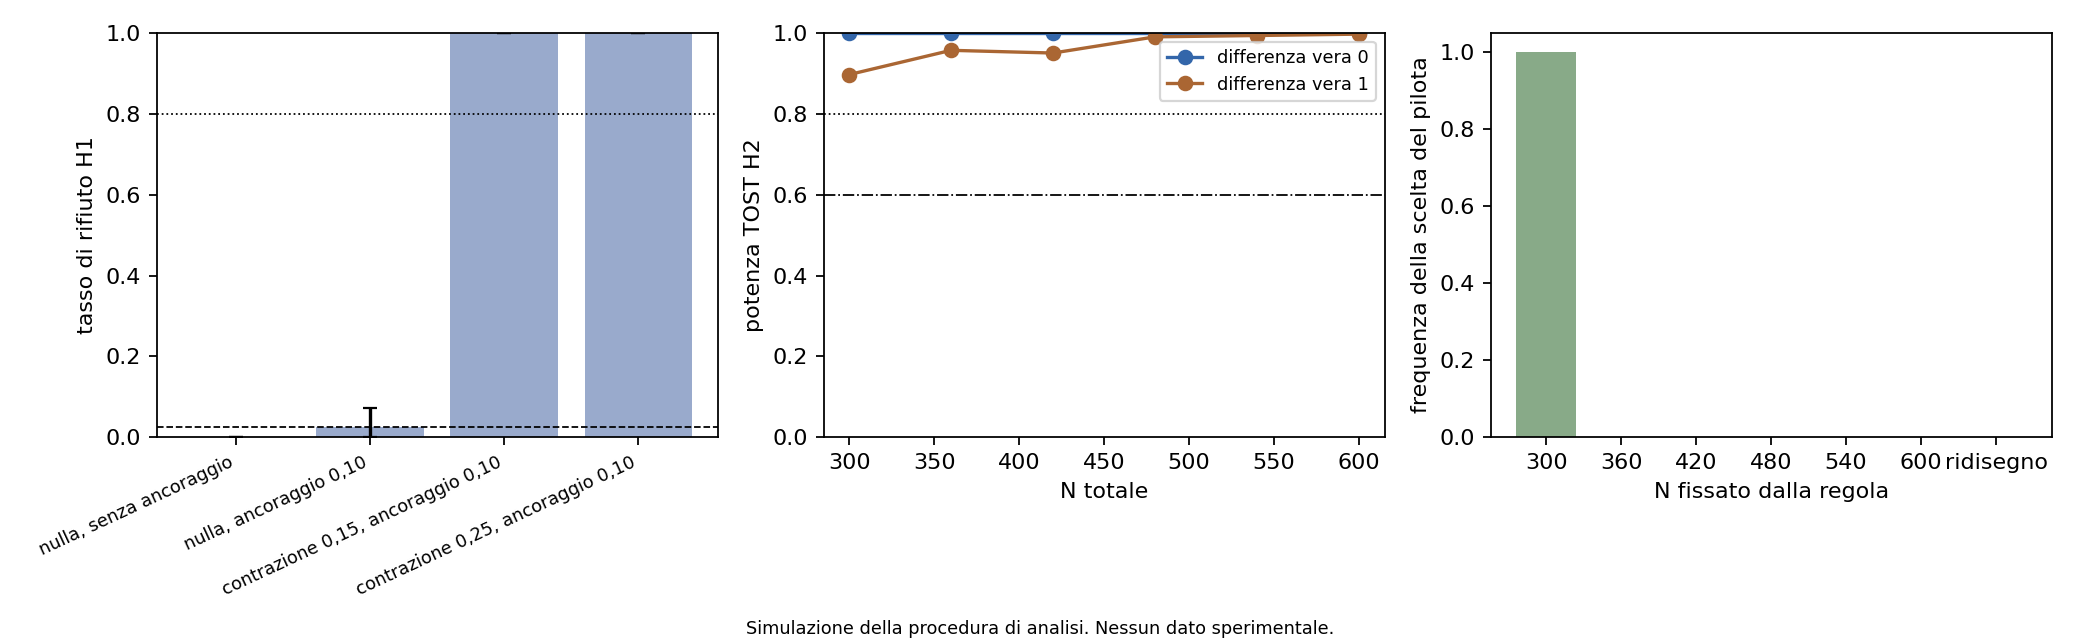
\includegraphics[width=\linewidth]{simulazione_completa.png}
\end{column}
\end{columns}
\end{frame}

\begin{frame}{What the simulation says about the sample}
\begin{center}
\begin{tabular}{lcccc}
\toprule
H2 scenario, 300 participants & $\delta=0$ & $\delta=1$ & implied SD & dyad ICC\\
\midrule
list noise 4, dyad effect 2 & 100\% & 89.7\% & 3.9 & 0.21\\
list noise 6, dyad effect 3 & 95.3\% & 79.0\% & 4.6 & 0.32\\
\bottomrule
\end{tabular}
\end{center}
\begin{itemize}
\item The planning base of 300 needs an individual standard deviation of about 5.9 or less. The structural model implies 3.9 to 4.6, so the pilot rule selects 300 in every simulated pilot.
\item The constraint binds only if the price instrument's own noise exceeds roughly eight points per list, which is exactly what the certain-value tasks in the pilot measure.
\item Dyad bootstrap and likelihood-ratio test agree on the example dataset (lower bound 0.10 for a true contraction of 0.15).
\item This is a design check with reduced replications. The certifying run of the dossier, 2,000 replications with type-one error tolerance 0.035, is scheduled for the pilot stage.
\end{itemize}
\end{frame}

\begin{frame}{Open points we would like your view on}
\begin{itemize}
\item \textbf{The equivalence margin.} Three points is five percent of the value distance. Is that the right notion of a negligible elicitation effect for this task?
\item \textbf{The programmed seller.} Removing the human counterpart makes the benchmark computable and follows Charness and Levin (2009). Is anything lost that matters for your reading of selection neglect?
\item \textbf{Running in class.} The design is calibrated on 300 external subjects with the lab-like online methodology of the CESARE group. A classroom run with students who study these very models would be a demonstration rather than data collection.
\item \textbf{Toward the final.} Preregistration draft in OSF format, lifting the zero error correlation between the two lists in the simulation, and the certifying 2,000-replication run.
\end{itemize}
\vfill
{\footnotesize Full dossier, documents and three verification programs reproducing every number shown here: github.com/francescopinna03/experimental\_counterpart}
\end{frame}

\end{document}
